\documentclass[../main.tex]{subfiles}

\begin{document}
	\section{Osservabilit\'a e ricostruibilit\'a}
		\[
			S:
			\begin{cases}
				\dot x &= Ax + Bu\\
				y &= Cx + Du
			\end{cases}
		\]
		Potremmo essere interessati a conoscere all'istante $ t $, lo stato $ x(t) $ o la condizione iniziale $ x(0^{-}) $, perch\'e $ x(t) $ pu\'o avere un significato fisico. Potremmo non averne una misura diretta. Inoltre posso voler utilizzare lo stato $ x(t) $ per esempio per fare feedback. Spesso (nella pratica sempre) ci si accontenta di una stima $ \hat x(t) $ dello stato.
		
		\begin{definition}
			Un sistema \'e completamente osservabile \textbf{se e solo se}, dati $ u(\tau) $ e $ y(\tau) $ per $ \tau \in [0,t] $, \'e possibile calcolare univocamente $ x(0^{-}) $.
		\end{definition}
	
		\begin{definition}
			Un sistema \'e completamente ricostruibile \textbf{se e solo se}, dati $ y(\tau) $ e $ u(\tau) $ per $ \tau \in [0,t] $, \'e possibile calcolare univocamente $ x(t) $.
		\end{definition}
	
		Poich\'e $ x(t) $ \'e sempre funzione della condizione iniziale $ x(0^{-}) $ e della sequenza di controllo $ u(\tau) $ con $ \tau \in [0,t] $, se un sistema \'e osservabile allora sar\'a anche ricostruibile. Non vale necessariamente il viceversa. Per i sistemi LTI a tempo continuo valgono entrambe le implicazioni:
		\begin{center}
			un sistema \'e osservabile $ \Leftrightarrow $ \'e ricostruibile.
		\end{center}
		Per dimostrarlo partiamo dall'equazione di Lagrange da cui \'e evidente che $ x(t) $ dipenda da $ x(0^{-}), u(.) $:
		\[
			x(t) = e^{At}x(0^{-}) + \int_{0^{-}}^{t} e^{A(t-\tau)} B\ u(\tau) d\tau
		\]
		ma poich\'e $ e^{At} $ \'e sempre invertibile $ \left( (e^{At})^{-1} = e^{-At} \right) $ otteniamo anche che la condizione iniziale $ x(0^{-}) $ dipende da $ x(t) $ e $ u(.) $:
		\begin{align*}
			e^{At} x(0^{-}) &= x(t) - \int_{0^{-}}^{t} e^{A(t-\tau)} B\ u(\tau) d\tau\\
			x(0^{-}) &= e^{-At} \left[ x(t) - \int_{0^{-}}^{t} e^{A(t-\tau)} B\ u(\tau) d\tau \right] 
		\end{align*}
		
		Consideriamo adesso l'uscita del sistema:
		\[
			y(t) = \underbrace{Ce^{At}x(0^{-})}_{y_l(t)} + \underbrace{\int_{0^{-}}^{t} e^{A(t-\tau)} B\ u(\tau) d\tau + Du(t)}_{y_f(t)}
		\]
		Se $ A, B, C, D $ e $ u(\tau) $ per $ \tau \in [0, t] $ sono noti, allora $ y_f(t) $ \'e calcolabile. $ y(t) $, essendo l'uscita del sistema, \'e nota perch\'e \'e misurabile. Quindi possiamo calcolare $ y_l(t) $ come:
		\[
			y_l(t) = y(t) - y_f(t)
		\]
		D'ora in poi supporremo di lavorare con il sistema "libero", cio\'e il sistema in cui l'uscita $ y_l(t) $ non \'e influenzata dall'ingresso, come se $ u(t) \equiv 0 $.
		\newline
		
		Supponiamo:
		\begin{itemize}
			\item
				$ \exists \tilde x\ \text{tale che se}\ x(0^{-}) = \tilde x \quad\Rightarrow\quad y_l(t) = \tilde y_l(t) \equiv 0 $\\
				cio\'e che esista uno stato $ \tilde x $ che dal punto di vista dell'uscita libera sia indistinguibile dall'origine (infatti se lo stato iniziale \'e l'origine $ x(0^{-}) $, l'uscita libera non pu\'o che essere nulla $ y_l(t) = 0 $).
			\item
				di avere $ x(0^{-}) = \hat x \quad\Rightarrow\quad y_l(t) = \hat y_l(t) $
			\item 
				di prendere uno stato iniziale $ x(0^{-}) = \hat x + \alpha \tilde x $ con $ \alpha \in \R $
		\end{itemize}
		Per il principio di sovrapposizione degli effetti:
		\[
			y_l(t) = \hat y_l(t) + \alpha \tilde y_l(t) = \hat y_l(t)
		\]
		Abbiamo che ottenuto che non possiamo distinguere univocamente lo stato iniziale partendo da $ y_l(t) $.
		
		\begin{definition}
			Definiamo $ X_{NO} $ l'insieme degli stati indistinguibili dallo stato zero:
			\[
				\tilde x \triangleq \left\lbrace \tilde x\ \text{tale che}\ x(0^{-}) = \tilde x \quad\Rightarrow\quad y_l(t) = 0 \right\rbrace
			\]
		\end{definition}
	
		Dalla conoscenza di $ \begin{cases} u(\tau)\\ y(\tau) \end{cases} \tau \in [0,t] $ non sar\'a possibile "osservare" univocamente $ x(0^{-}) $, ma solo una variazione di $ x(0^{-}) $ a meno di $ X_{NO} $.
		
		\paragraph{Propriet\'a di $ X_{NO} $:}
			\begin{itemize}
				\item 
					$ X_{NO} $ \'e un sottospazio lineare: se $ \tilde x_1 \in X_{NO} $ e $ \tilde x_2 \in X_{NO} $, allora $ \alpha \tilde x_1 + \beta x_2 \in X_{NO} $
				\item 
					$ X_{NO} $ \'e invariante rispetto ad $ A $: se $ \tilde x \in X_{NO} $, allora $ A \tilde x \in X_{NO} $
			\end{itemize}
	
	\subsection{Teorema di Kalmann di Osservabilit\'a}
		\[
			X_{NO} \triangleq Ker\{Q\} \quad n_{NO} \triangleq dim { X_{NO} }
		\]
		\[
			Q \triangleq
			\underbrace{
				\left. 
				\begin{bmatrix}
					C\\
					CA\\
					CA^2\\
					\vdots\\
					CA^{n_x-1}
				\end{bmatrix}
			\right\rbrace 
			}_{n_x}
			n_x \times n_y
		\]
	\subsection{Corollari del teorema di Kalmann}
		\begin{itemize}
			\item
				\textbf{sistema completamente osservabile} $ \quad\Leftrightarrow\quad $
				\[
					\quad\Leftrightarrow\quad X_{NO} = Ker\{Q\} = {0} \quad\Leftrightarrow\quad n_{NO} = 0 \quad\Leftrightarrow\quad rank\{Q\} = n_x\ \text{(ha rango massimo)}
				\]
			\item 
				posso applicare il teorema di Kalmann di osservabilit\'a a gruppi di uscite o a ogni singola uscita.
			\item 
				sistema completamente non osservabile $ \quad\Leftrightarrow\quad X_{NO} = \R^{n_x} \quad\Leftrightarrow\quad rank\{Q\} = 0 \quad\Leftrightarrow\quad C = [0] $ cio\'e l'uscita non dipende dallo stato.
		\end{itemize}
	
		\hrule
		\begin{Exercise}[title={Calcolare $ X_{NO} $}, difficulty=1]
		\hrule\medskip
			\[
				\dot x =
				\begin{bmatrix}
					-1 & 0 & 0\\
					0 & 0 & 1\\
					0 & 1 & 0
				\end{bmatrix} x + Bu
				\qquad
				y =
				\begin{bmatrix}
					1 & 0 & 0\\
					0 & 0 & 1
				\end{bmatrix} x
			\]
			\[
				Q =
				\begin{bmatrix}
					C\\
					CA\\
					CA^2 = (CA)A
				\end{bmatrix} =
				\begin{bmatrix}
					1 & 0 & 0\\
					0 & 0 & 1\\
					\hline
					-1 & 1 & 0\\
					0 & 1 & 0\\
					\hline
					1 & 0 & 0\\
					0 & 1 & 0
				\end{bmatrix}
			\]
			$ rank\{Q\} = 3 = n_x $ il rango \'e massimo quindi il sistema \'e completamente osservabile.
			
			Consideriamo solo l'uscita $ y_1 $:
			\[
				C_1 =
				\begin{bmatrix}
					1 & 0 & 0
				\end{bmatrix}
				\quad\Rightarrow\quad
				Q_1 =
				\begin{bmatrix}
					1 & 0 & 0\\
					-1 & 1 & 0\\
					1 & 0 & 0
				\end{bmatrix}
			\] 
			$ rank\{Q_1\} = 2 $ quindi il sistema non \'e completamente osservabile da $ y_1 $. Calcoliamo $ X_{NO1} $:
			\[
				\tilde x =
				\begin{bmatrix}
					a\\
					b\\
					c
				\end{bmatrix}
				\quad\text{tale che}\quad
				Q_1 \tilde x = 0
			\]
			\[
				\begin{bmatrix}
					1 & 0 & 0\\
					-1 & 1 & 0\\
					1 & 0 & 0
				\end{bmatrix}
				\begin{bmatrix}
					a\\
					b\\
					c
				\end{bmatrix} =
				\begin{bmatrix}
					0\\
					0\\
					0
				\end{bmatrix}
				\quad\Rightarrow\quad
				\begin{cases}
					a = 0\\
					-a+b = 0\\
					a = 0
				\end{cases}
				\quad\Rightarrow\quad X_{NO} =
				\begin{bmatrix}
					0\\
					0\\
					c
				\end{bmatrix}
			\]
			Consideriamo solo $ y_2 $:
			\[
				C_2 =
				\begin{bmatrix}
					0 & 0 & 1
				\end{bmatrix}
				\quad\Rightarrow\quad
				Q_2 =
				\begin{bmatrix}
					0 & 0 & 1\\
					0 & 1 & 0\\
					0 & 1 & 0
				\end{bmatrix}
			\] 
			$ rank\{Q_2\} = 2 $ quindi il sistema non \'e completamente osservabile da $ y_2 $. Calcoliamo $ X_{NO2} $ analogamente a prima e otteniamo:
			\[
				X_{NO2} = Ker\{Q_2\} =
				\begin{bmatrix}
					a\\
					0\\
					0
				\end{bmatrix}
			\]
			\hrule
		\end{Exercise}
	
	\subsection{Decomposizione di Kalmann di osservabilit\'a}
		Prendiamo una matrice $ T = [T_1 | T_2] $ dove
		\begin{itemize}
			\item 
				$ T_1 $ \'e una matrice le cui colonne sono base di $ X_{NO} $
			\item
				$ T_2 $ \'e una matrice le cui colonne sono base di $ X_O \triangleq X_{NO}^{\perp} $
		\end{itemize}
		Effettuiamo il cambio di base: $ x = Tz $:
		\[
			\begin{cases}
				\dot z = T^{-1}ATz + T^{-1}Bu\\
				y = CTz + Du
			\end{cases}
		\]
		Si pu\'o dimostrare che:
		\[
			\begin{cases}
				\dot z =
				\begin{bmatrix}
					\dot z_O\\
					\dot z_{NO}
				\end{bmatrix} =
				\begin{bmatrix}
					\tilde A_{11} & 0\\
					\tilde A_{21} & \tilde A_{22}
				\end{bmatrix}
				\begin{bmatrix}
					z_O\\
					z_{NO}
				\end{bmatrix}
				+ Bu
				\\[.5cm]
				y =
				\begin{bmatrix}
					\tilde C_1 & 0
				\end{bmatrix}
				\begin{bmatrix}
					z_{O}\\
					z_{NO}
				\end{bmatrix}
				+ Du
			\end{cases}
		\]
		dove $ z_{NO} $ \'e la componente dello stato non osservabile (perch\'e non influenza $ y $ n\'e direttamente n\'e indirettamente attraverso $ z_O $), mentre $ z_O $ \'e la componente osservabile. Quindi sar\'a possibile calcolare solo $ z_O(0^{-}) $.
		
		\begin{figure}[H]
			\centering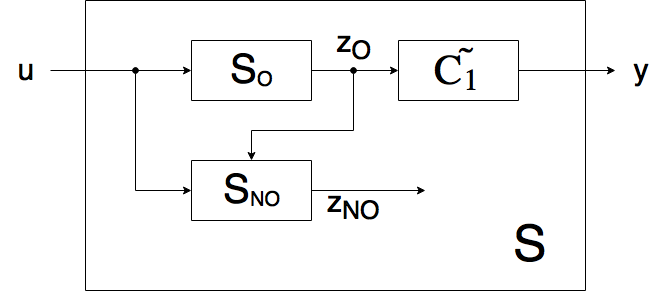
\includegraphics[width=.5\textwidth]{osservabilita_ricostruibilita/decomposizione_osservabilita}
		\end{figure}
		
	\subsection{Polinomio caratteristico di osservabilit\'a}
		\[
			\varphi(s) = \tilde{\varphi}(s) = \underbrace{det(sI- \tilde A_{11})}_{\varphi_O(s)} \cdot \underbrace{det(sI- \tilde A_{22})}_{\varphi_{NO}(s)}
		\]
		\begin{itemize}
			\item 
				$ \varphi_O(s) $ \'e il polinomio caratteristico di osservabilit\'a: ha come radici gli autovalori di $ \tilde A_{11} $ e sono detti autovalori osservabili.
			\item 
				$ \varphi_{NO}(s) $ \'e il polinomio caratteristico di non osservabilit\'a: ha come radici gli autovalori di $ \tilde A_{22} $ e sono detti autovalori di non osservabilit\'a.
		\end{itemize}
	
	\subsubsection{Come calcolare gli autovalori osservabili}
		\begin{align*}
			y_l(t) &= C e^{At} x(0^{-}) = \tilde C e^{\tilde At} z(0^{-})\\
			\intertext{trasformiamo con Laplace:}
			Y_l(s) &= C(sI-A)^{-1}x(0^{-}) = \tilde C (sI-\tilde A)^{-1} z(0^{-})
		\end{align*}
		\begin{align*}
			\tilde C (sI-\tilde A)^{-1} =
			\begin{bmatrix}
				\tilde C_1 & 0
			\end{bmatrix}
			\begin{bmatrix}
				sI-\tilde A_{11} & 0\\
				-\tilde A_{21} & sI-\tilde A_{22}
			\end{bmatrix}^{-1} =
			\\
			\begin{bmatrix}
				\tilde C_1 & 0
			\end{bmatrix}
			\begin{bmatrix}
				(sI-\tilde A_{11})^{-1} & 0\\
				-\tilde A_{21} & (sI-\tilde A_{22})^{-1}
			\end{bmatrix} =
			\begin{bmatrix}
				\tilde C_1 (sI- \tilde A_{11})^{-1} & 0
			\end{bmatrix}
		\end{align*}
		\begin{align*}
			\Rightarrow\quad Y_l(s) &=
			\begin{bmatrix}
				\tilde C_1(sI-\tilde A_{11})^{-1} & 0
			\end{bmatrix}
			\begin{bmatrix}
				z_O\\
				z_{NO}
			\end{bmatrix} =
			\\
			&= \tilde C_1 (sI-\tilde A_{11})^{-1} z_O(0^{-}) + 0 \cdot z_{NO}(0^{-}) =
			\\
			\intertext{ma per quanto detto prima}
			&= C(sI-A)^{-1} x(0^{-})
		\end{align*}
		
		Gli autovalori osservabili sono quelli che caratterizzano, con la loro molteplicit\'a, tutte le possibili uscite (i modi di evoluzione dell'uscita) al variare di $ x(0^{-}) $. $ \varphi_O(s) $ pu\'o essere ottenuto come polinomio caratteristico associato a $ \tilde C (sI-\tilde A)^{-1} $ o equivalentemente a $ C(sI-A)^{-1} $.\\
		(Un discorso analogo vale per il polinomio minimo $ m_O(s) \subseteq \cdot \varphi_O(s) $).
		\[
			\text{sistema completamente osservabile} \quad\Leftrightarrow\quad \pDeg{\varphi_O(s)} = n_x \quad\text{cioe\'e se}\ \varphi_O(s) \equiv \varphi(s)
		\]
		
	\subsection{Studio dell'osservabilit\'a}
		\begin{itemize}
			\item 
				Utilizzando il teorema di Kalmann si trovano $ X_{NO} $ e $ n_O = n_x - dim(X_{NO}) $
			\item 
				Studiando $ C(sI-A)^{-1} $ si ottengono $ \varphi_O(s) $ e $ \pDeg{\varphi_O(s)} $
		\end{itemize}
		Entrambi i metodi hanno in comune:
		\[
			n_O = dim(X_O) = n_x - dim(X_{NO}) = \pDeg{\varphi_O(s)}
		\]
		
		\begin{Exercise}[title={Studiare l'osservabilit\'a di due vasche in parallelo}]
			Consideriamo la linearizzazione del sistema attorno a un punto di equilibrio:
			\[
				\begin{cases}
					\dot x=
					\begin{bmatrix}
						-\alpha_1 & 0\\
						0 & -\alpha_2
					\end{bmatrix} x + Bu	
					\\
					y = S_1 x_1 + S_2 x_2
				\end{cases}
			\]
			\begin{itemize}
				\item 
					$ \alpha_1 = \dfrac{E_1}{2S_1} \sqrt{\dfrac{2g}{\bar h_1}} \qquad \alpha_2 = \dfrac{E_2}{2S_2} \sqrt{\dfrac{2g}{\bar h_2}} $ 
				\item 
					$ x_1 \triangleq h_1 - \bar h_1 \qquad x_2 \triangleq h_2 - \bar h_2 $\\
					rappresenta la variazione di altezza del volume d'acqua nella vasca rispetto il livello del punto di equilibrio. \'E una quantit\'a che possiamo conoscere ad esempio misurandola con un galleggiante.
				\item 
					$ y $ \'e la somma delle variazioni di volume delle vasche rispetto al loro punto di equilibrio. Anch'essa \'e una quantit\'a misurabile per esempio con una bilancia sotto le due vasche. 
			\end{itemize}
		
			Studiamo l'osservabilit\'a del sistema, cio\'e se \'e possibile ricavare il volume di ciascuna vasca partendo dal volume totale.
			
			\paragraph{Metodo con teorema di Kalmann}
				\[
					Q =
					\begin{bmatrix}
						S_1 & S_2\\
						-\alpha_1 S_1 & -\alpha_2 S_2
					\end{bmatrix}
				\]
				\[
					det\left\lbrace Q \right\rbrace = -\alpha_2 S_1 S_2 + \alpha_1 S_1 S_2 = S_1 S_2 (\alpha_1 - \alpha_2)
				\]
				
				\begin{itemize}
					\item 
						se $ \alpha_1 \neq \alpha_2 $ il sistema \'e osservabile posso risalire al volume delle vasche partendo dal modo di evoluzione dell'uscita $ y $.
					\item 
						se $ \alpha_1 = \alpha_2 = \alpha $ il sistema non \'e osservabile.
				\end{itemize}
			
				In quest'ultimo caso calcoliamo $ X_{NO} $:
				\[
					\tilde x =
					\begin{bmatrix}
						a\\
						b
					\end{bmatrix} \in X_{NO}
					\quad\Leftrightarrow\quad 
					\begin{bmatrix}
						S_1 & S_2\\
						-\alpha_1 S_1 & -\alpha_2 S_2
					\end{bmatrix}
					\begin{bmatrix}
						a\\
						b
					\end{bmatrix} =
					\begin{bmatrix}
						0\\
						0
					\end{bmatrix}
				\]
				\[
					\Rightarrow\quad aS_1 + bS_2 = 0 \quad\Rightarrow\quad b = -\dfrac{S_1}{S_2}a \quad\Rightarrow\quad X_{NO} =
					\begin{bmatrix}
						a\\
						-\dfrac{S_1}{S_2}a
					\end{bmatrix}
				\]
				
				Significa che se il sistema si trova nella situazione in cui:
				\begin{itemize}
					\item 
						il livello della prima vasca \'e $ \bar h + a $;
					\item 
						il livello della seconda vasca \'e $ \bar h - \dfrac{S_1}{S_2}a $;
					\item 
						applichiamo il controllo $ \bar u $ del punto di equilibrio
				\end{itemize}
				e misuriamo il volume delle due vasche attraverso la "bilancia", otteniamo un valore costante $ (y_l = 0) $, anche se lo stato del sistema sta variando.
				
			\paragraph{Metodo con polinomio caratteristico}
				\[
					C(sI-A)^{-1} =
					\begin{bmatrix}
						S_1 & S_2
					\end{bmatrix}
					\begin{bmatrix}
						\dfrac{1}{s+\alpha_1} & 0\\
						0 & \dfrac{1}{s+\alpha_2}
					\end{bmatrix} =
					\begin{bmatrix}
						\dfrac{S_1}{s+\alpha_1} & \dfrac{S_2}{s+\alpha_2}
					\end{bmatrix}
				\]
				\[
					\varphi_O(s) = mcm\left\lbrace (s+\alpha_1), (s+\alpha_2) \right\rbrace =
					\begin{cases}
						(s+\alpha) \qquad\text{se}\ \alpha_1 = \alpha_2 = \alpha\\
						(s+\alpha_1)(s+\alpha_2) \qquad\text{se}\ \alpha_1 \neq \alpha_2
					\end{cases}
				\]
				
				Calcoliamo la trasformata di Laplace dell'uscita:
				\[
					Y(s) = C(sI-A)^{-1} x(0^{-}) = \dfrac{S_1}{s+\alpha_1}x_1(0^{-}) + \dfrac{S_2}{s+\alpha_2}x_2(0^{-})
				\]
				\[
					y(t) = S_1x_1(0^{-}) e^{-\alpha_1 t} + S_2x_2(0^{-}) e^{-\alpha_2 t}
				\]
				
				Nel caso non osservabile $ \alpha_1 = \alpha_2 = \alpha $:
				\[
					Y(s) = [S_1 x_1(0^{-}) + S_2 x_2(0^{-})] \dfrac{1}{s+\alpha}
				\]
				\[
					y(t) = [S_1 x_1(0^{-}) + S_2 x_2(0^{-})] e^{-\alpha t}
				\]
				Poich\'e il sistema non \'e osservabile non possiamo ottenere $ x_1(0^{-}) $ e $ x_2(0^{-}) $ separatamente, ma solo $ \left[ S_1 x_1(0^{-}) + S_2 x_2(0^{-}) \right] $.
			
			\paragraph{Sistema con due uscite}
				Consideriamo adesso il caso in cui abbiamo due misure:
				\[
					\begin{cases}
						y_1 = x_1\\
						y_2 = x_2
					\end{cases}
					\quad\Rightarrow\quad
					C =
					\begin{bmatrix}
						1 & 0\\
						0 & 1
					\end{bmatrix}
				\]
				Si vede subito che il sistema \'e completamente osservabile perch\'e lo stato coincide con le uscite, ma si pu\'o ricavare rigorosamente con il teorema di Kalmann: basta osservare che $ rank\left\lbrace C \right\rbrace = 2 = n_x $.
				
				La trasformata dell'uscita nel caso $ \alpha_1 = \alpha_2 = \alpha $ \'e:
				\[
					Y(s) = C(sI-A)^{-1} x(0^{-}) =
					\begin{bmatrix}
						\dfrac{1}{s+\alpha} & 0\\
						0 & \dfrac{1}{s+\alpha}
					\end{bmatrix} x(0^{-}) =
					\begin{bmatrix}
						\dfrac{1}{s+\alpha} x_1(0^{-})\\
						\dfrac{1}{s+\alpha} x_2(0^{-})
					\end{bmatrix}
				\]
				\[
					\varphi_O(s) = mcm\left\lbrace (s+\alpha), (s+\alpha), (s+\alpha)^2 \right\rbrace = (s+\alpha)^2
				\]
				
				Nonostante abbiamo un solo autovalore $ s = \alpha $ con molteplicit\'a $ 2 $, il sistema \'e comunque osservabile, grazie al fatto che si hanno due uscite.
		\end{Exercise}
\end{document}